\documentclass{article}
\usepackage{graphicx}
\usepackage[margin = 1.2in]{geometry}
\usepackage{amsmath}

\begin{document}

For the following system of ODE's,

\begin{align} \label{sys:ODE}
  c' &= -\frac{\mu}{y} \frac{cx}{k_1 +c} - \frac{\eta}{y} \frac{cax}{k_2 +c} + q(c_0 - c) \\
  a' &= -\frac{\eta}{z} \frac{cax}{k_2+c} + q (a_0 -a)\\
  x' &= \mu \frac{cx}{k_1+c} - \eta \frac{cax}{k_2+c} - qx\\
  p' &= \frac{cx}{k_1 +c},
\end{align}

using the following parameter values,

\begin{center}
  \begin{tabular}{c|c}
    Parameter & Value \\
    \hline
    $\mu$ & 2 \\
    $y$ & 1\\
    $k_1$ & 1.5\\
    $k_2$ & 1.5\\
    $\eta$ & 10 \\
    $q$ & 0.2 \\
    $c_0$ & 1\\
    $a_0$ & 1\\
    $z$ & 1,
  \end{tabular}
\end{center}

I graphed out how the system behaves when the antibodies, $a$, are introduced. To simulate this effect, the equation for $a'$ was changed to

\begin{align}
  \alpha' = -\frac{\eta}{z} \frac{cax}{k_2+c} + q (a_\infty &-a) (h(t_{start},t) - h(t_{end},t)) \\
  \text{with } h(x,y) &= \frac{x^n}{y^n + x^n} \\
  \text{and } t_{start} &= 10, \\
  t_{end} &= 15,\\
  n &= 100. 
\end{align}

With this change it can be said that $\alpha'(x) = a'(x), \forall x, 10 \le x \le 15$. The graphs can be seen in Figure \ref{eqsVsTime} and in Figure \ref{phase:xc}.

\begin{center}
  \begin{figure}
    \begin{tabular}{cc}
      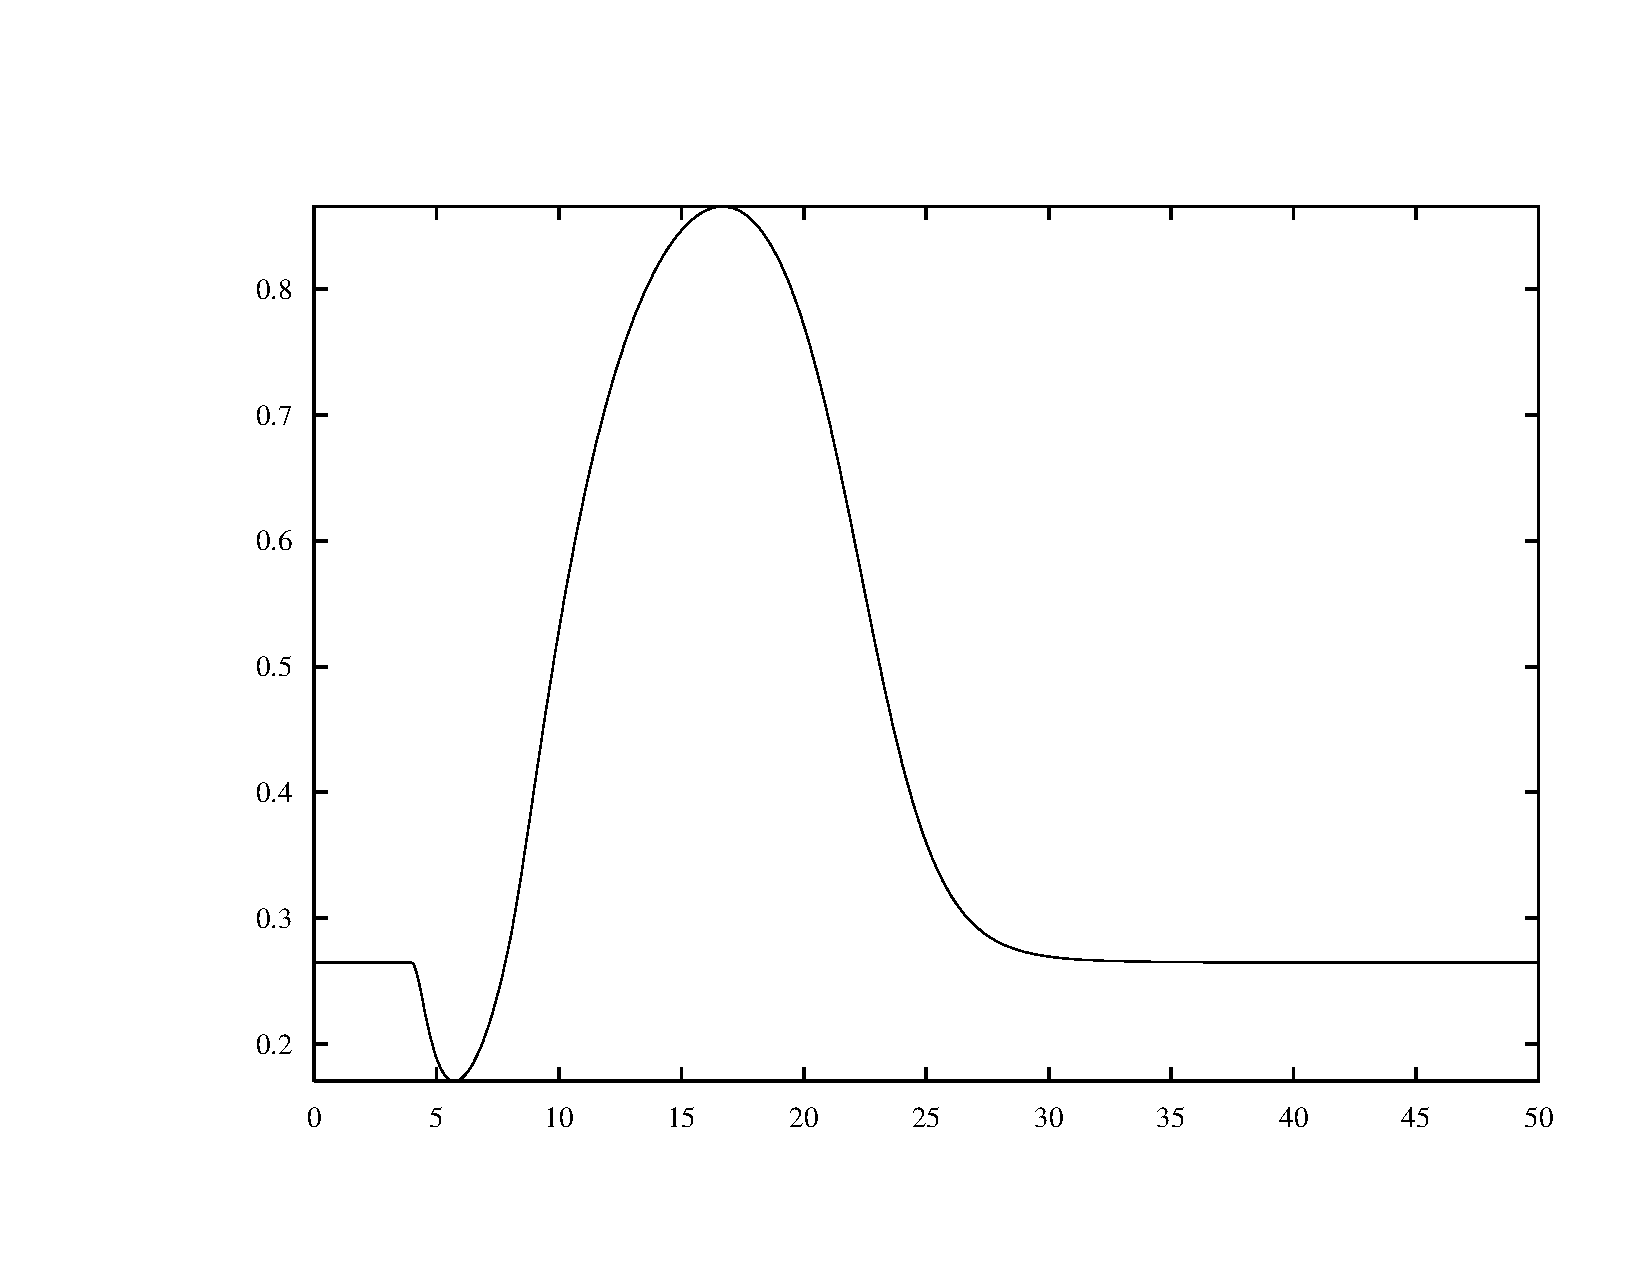
\includegraphics[scale = 0.3, angle = 0]{carbonTime.pdf} &
      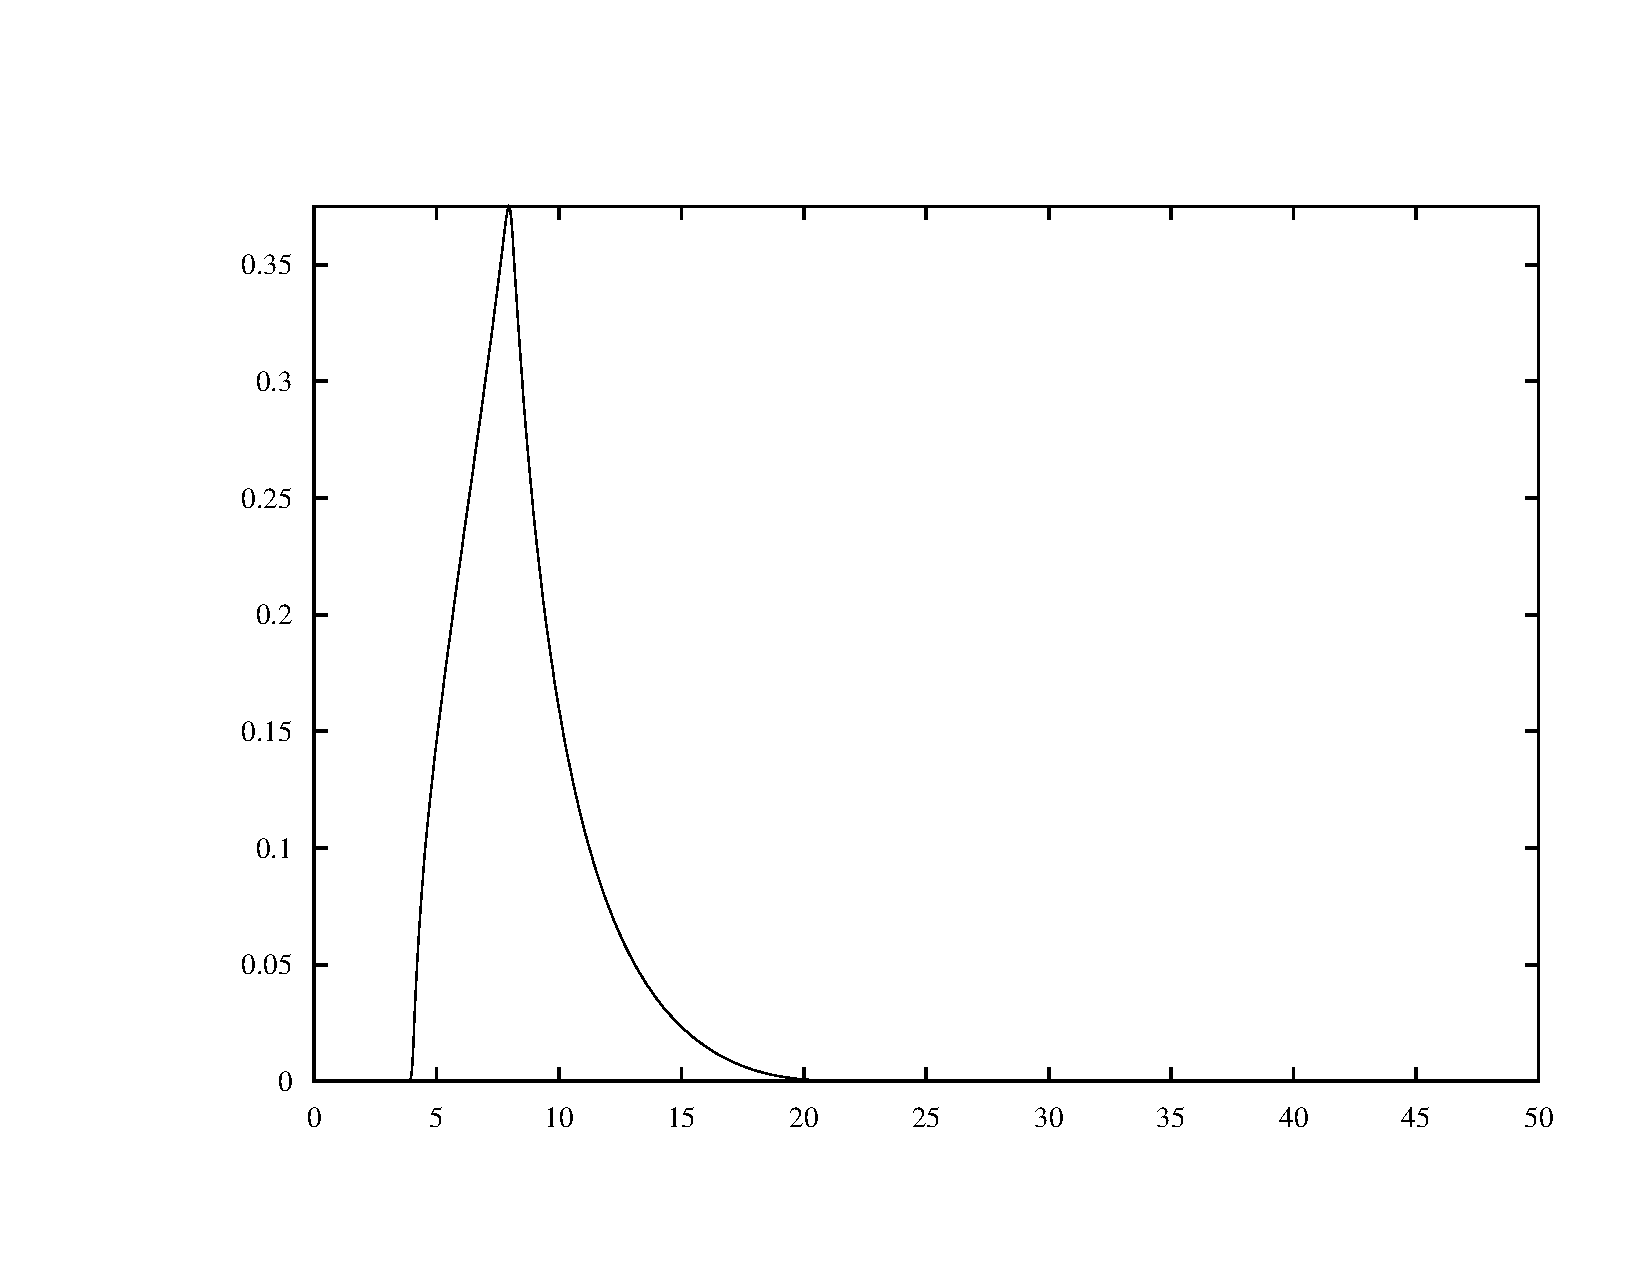
\includegraphics[scale = 0.3, angle = 0]{antiTime.pdf}  \\
      (a) & (b) \\
      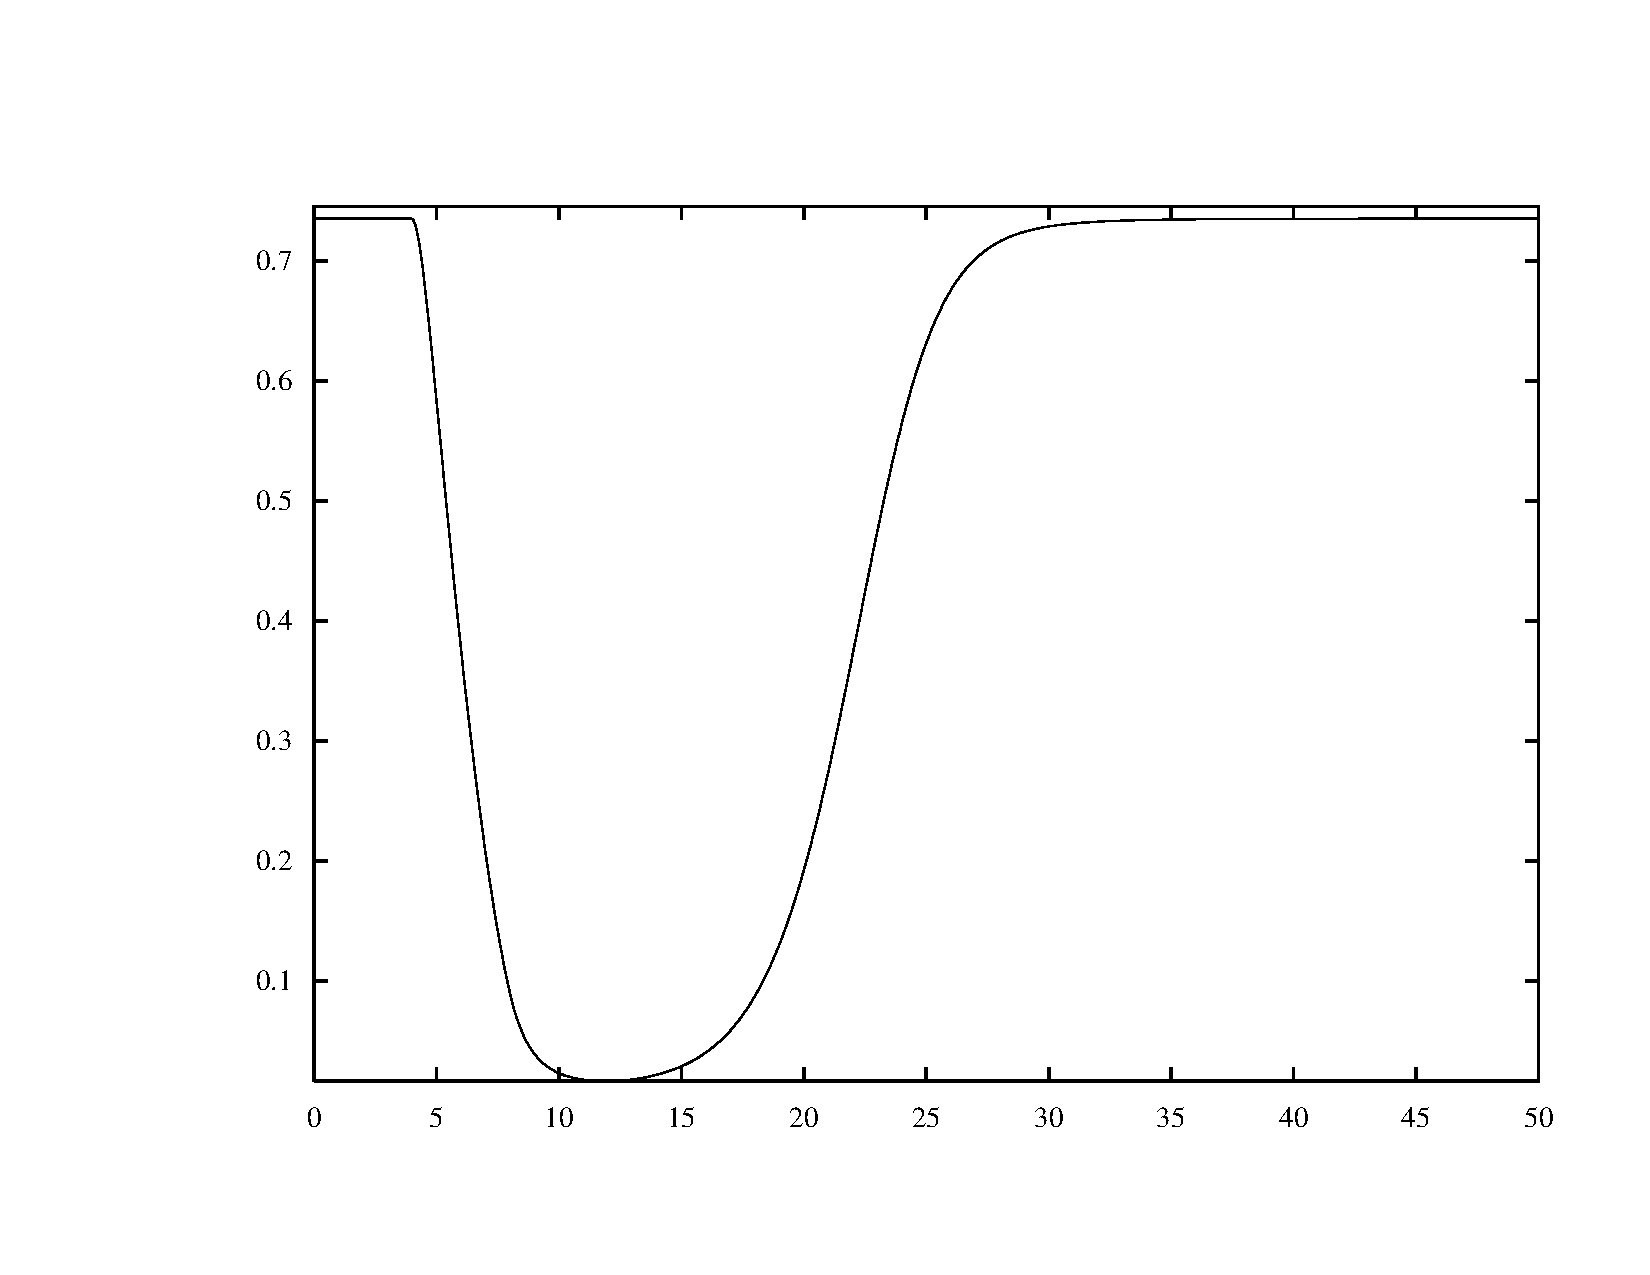
\includegraphics[scale = 0.3, angle = 0]{bactTime.pdf} &
      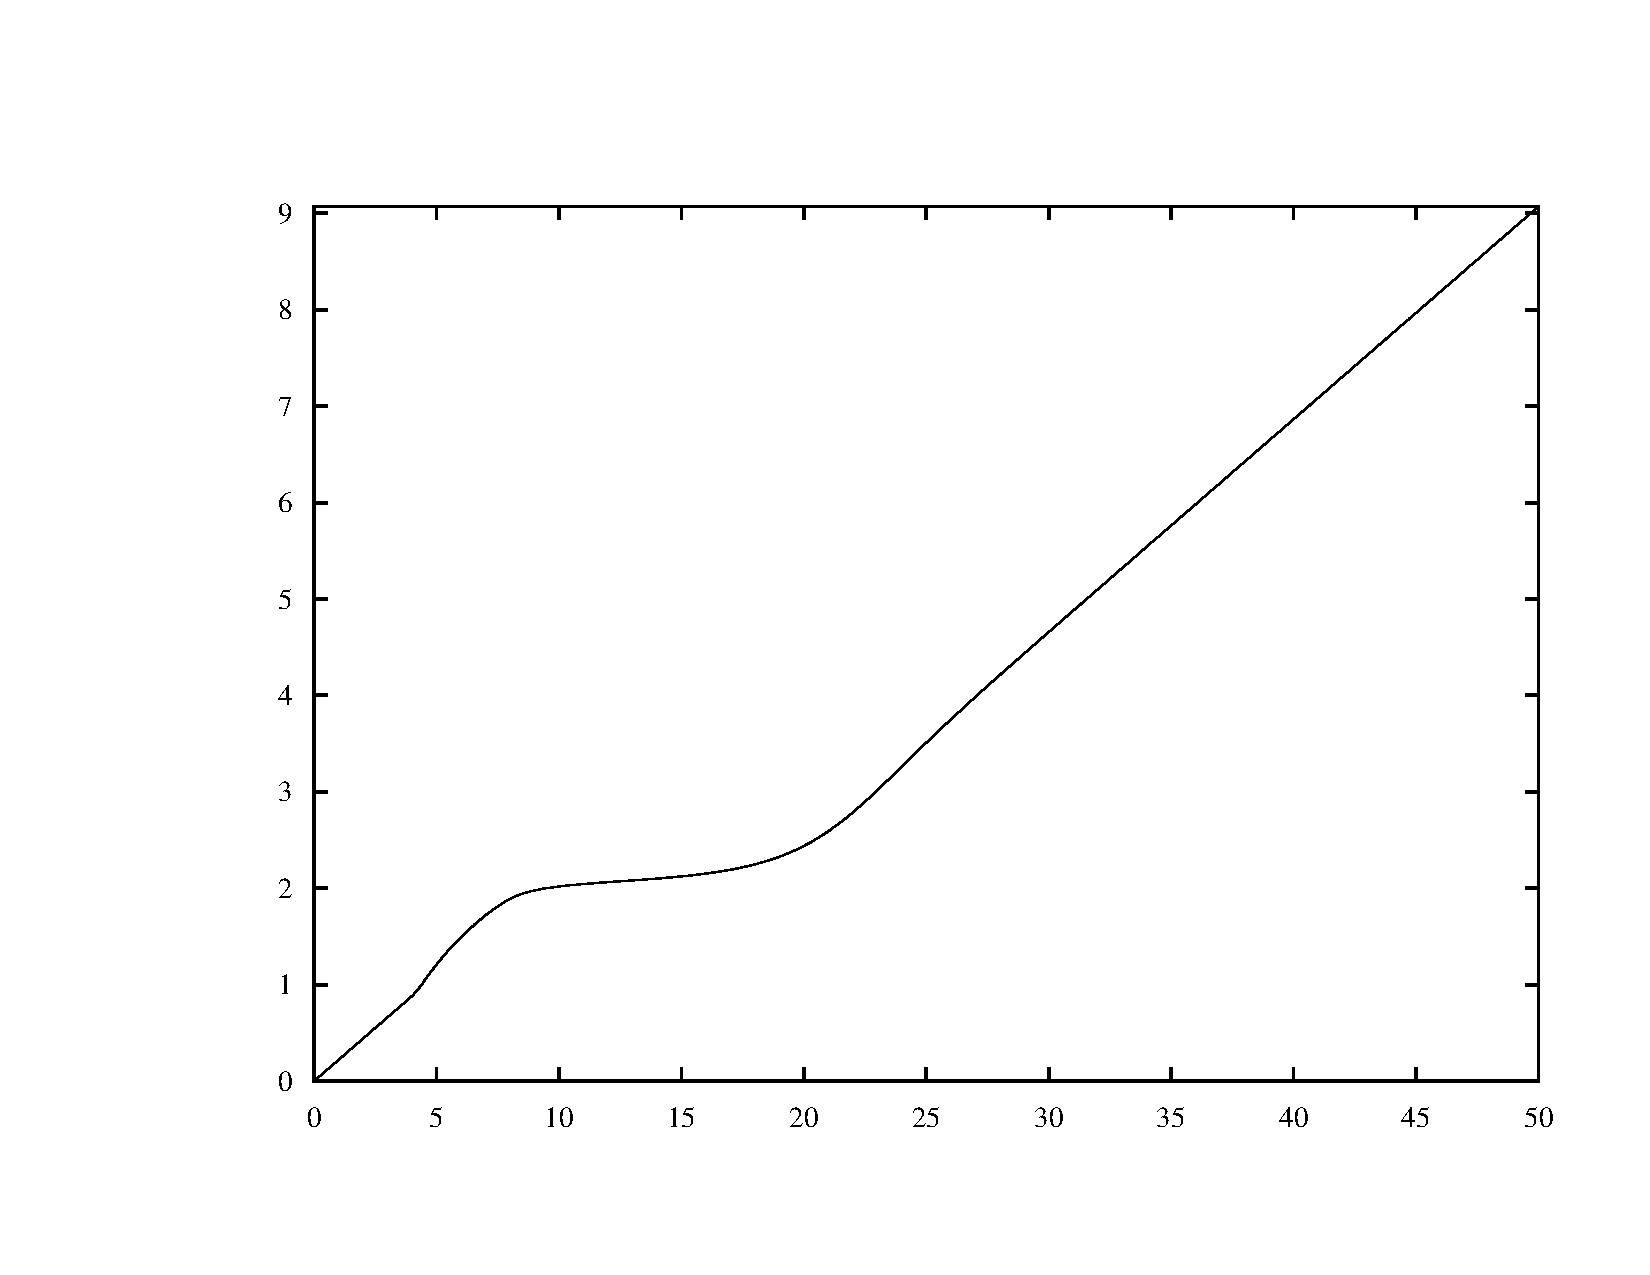
\includegraphics[scale = 0.3, angle = 0]{biprodTime.pdf}\\
      (c) & (d)
    \end{tabular}
    \caption{(a) $c$ vs. time (b) $a$ vs. time (c) $x$ vs. time (d) $p$ vs. time}
    \label{eqsVsTime}
  \end{figure}
\end{center}

\begin{center}
\begin{figure}
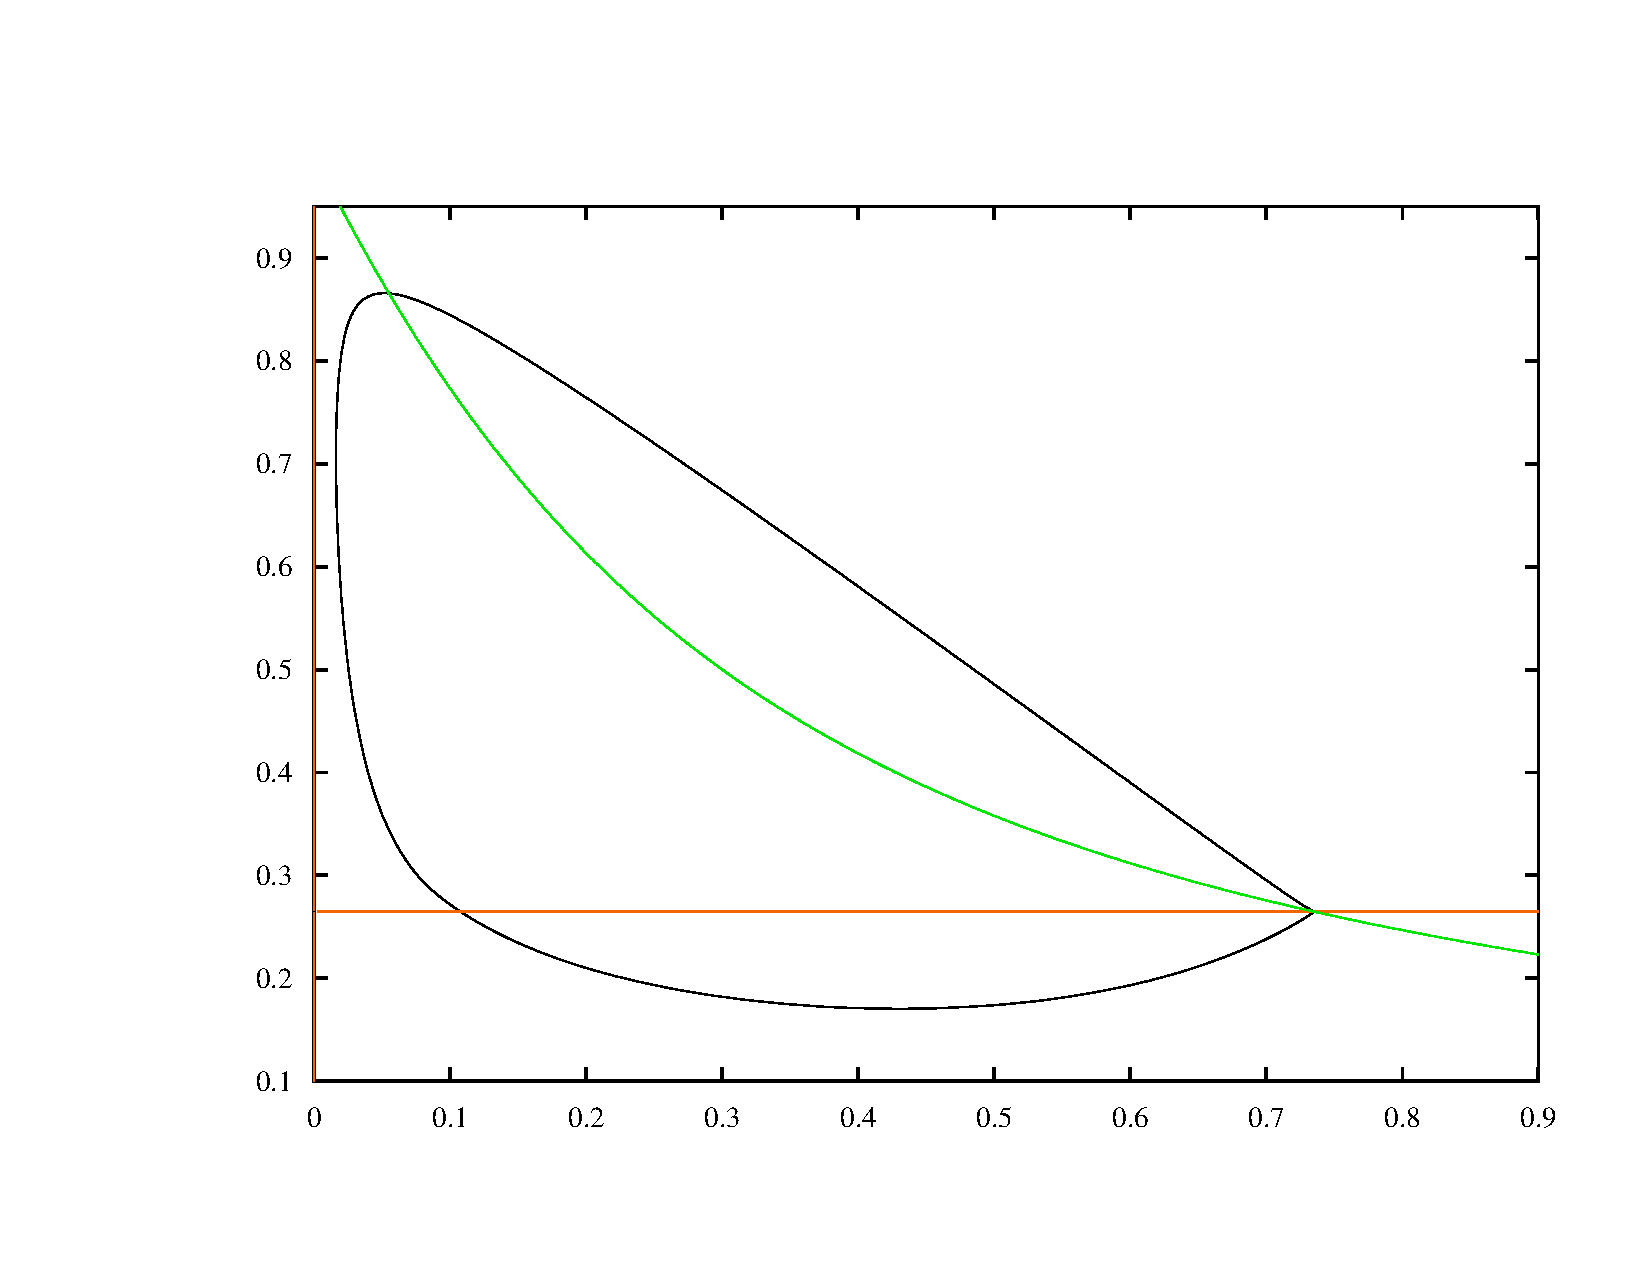
\includegraphics[scale = 0.5]{carbonBact.pdf}
\caption{Phase portrait of $x$ and $c$}
\label{phase:xc}
\end{figure}
\end{center}

The effect of replacing $\frac{cax}{k_2 +c}$ with $\frac{k_2 cax}{(k_1+c)(k_2+c)}$ in (\ref{sys:ODE})-(4) was examined. It was determined that there is no noticable effect from this change.


\end{document}




